\section{Cross talk measutrements}

Electronic crosstalk is present in both the H12700 and H8500 MAPMTs. This can be observed by plotting the measured charge in one pixel vs. the measured charge in an adjacent pixel. Fig.~\ref{fig:H12700neighbors} and Fig.~\ref{fig:H8500neighbors} show these two dimensional plots for all pixels which neighbor pixel 28 for one H12700 MAPMT and one H8500 MAPMT, respectively. The crosstalk bands are most prominently seen in the pixels directly to the left or right, where the amount of crosstalk is shown to be proportional to the charge measured in the central pixel. 


\begin{figure*}
	\centering
	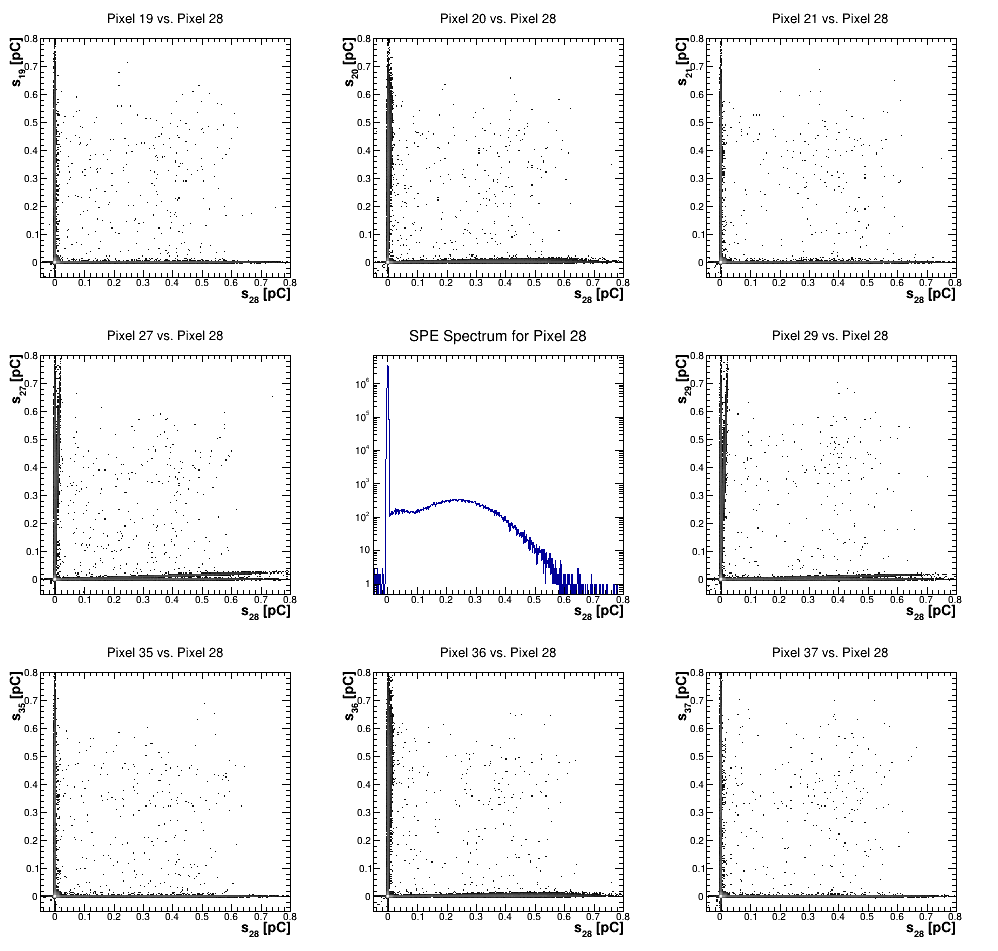
\includegraphics[width=0.95\linewidth]{figures/GA0982_neighbors_crosstalk.png}
	\caption{}
	\label{fig:H12700neighbors}
\end{figure*}
\begin{figure*}
	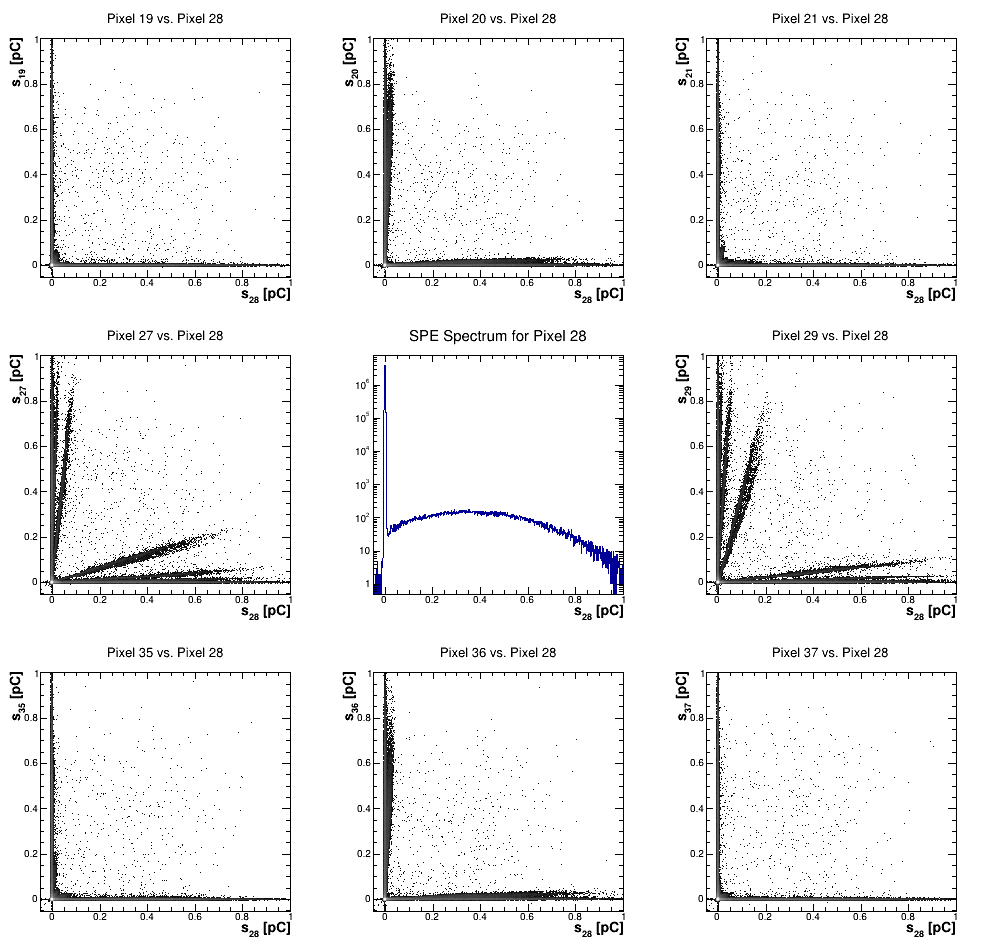
\includegraphics[width=0.95\linewidth]{figures/CA7709_neighbors_crosstalk.png}
	\caption{}
	\label{fig:H8500neighbors}
\end{figure*}


\subsection{Offline Crosstalk Removal}

A simple method was developed to remove the crosstalk offline on an event-by-event basis. Crosstalk events in neighboring pixels are characterized by bands in the two dimensional plots showing the measured charge in one pixel against the maximum measured charge in the neighboring pixels. In cases where light only entered the central pixel, the neighboring pixels may have some non-zero signal which should be proportional to the amount of charge collected in the central pixel. This can be seen in the example shown below which plots the maximum charge measured in the neighboring pixels of 
